%% Artigo, versão 2 — template IEEE de conferência (IEEEtran), esqueleto de report/draft_final_rascunho
%% fundido com report/artigo_v1. Compilar a partir desta pasta:  pdflatex main && pdflatex main
%% Números de report/resultados_benchmark_obstrucao.md, report/resultados_benchmark_manipulacao.md,
%% report/analise_fp_fn_manipulacao.md e das saídas de notebooks/benchmark_manipulacao.ipynb
%% (execução de 16-17/11/2026); não recalculados aqui. Figuras: draft_final_rascunho/figures e
%% artigo_v1/figures.
\documentclass[conference]{IEEEtran}

\usepackage[utf8]{inputenc}
\usepackage[T1]{fontenc}
\usepackage[brazil]{babel}
\usepackage{cite}
\usepackage{amsmath,amssymb,amsfonts}
\usepackage{graphicx}
\usepackage{textcomp}
\usepackage{xcolor}
\usepackage{booktabs}
\usepackage{multirow}
\usepackage{array}
\usepackage{tikz}
\usetikzlibrary{arrows.meta,positioning,calc}
\usepackage{url}
\usepackage[hidelinks]{hyperref}

\graphicspath{{figures/}}
\newcolumntype{L}[1]{>{\raggedright\arraybackslash}p{#1}}
\newcommand{\Ir}{I_r}
\newcommand{\Ia}{I_a}
\newcommand{\Ageo}{A_{\mathrm{geo}}}
\newcommand{\var}[1]{\texttt{#1}}
\newcommand{\vpaper}{\var{paper}}
\newcommand{\vneutral}{\var{neutral}}
\newcommand{\vpd}{\var{paper\_\allowbreak decomposed}}
% Caixa para trechos de resposta dos modelos: #1 = quem respondeu, #2 = trecho.
\newcommand{\vlmbox}[2]{\par\smallskip\noindent\fbox{\begin{minipage}{\dimexpr\linewidth-2\fboxsep-2\fboxrule\relax}
\scriptsize\textsf{\textbf{#1}}\\[1pt]\ttfamily\raggedright #2\end{minipage}}\par\smallskip}

\hyphenation{Grounding ViDDAR VIM-Sense LLaVA Qwen Gemma}
\renewcommand{\IEEEkeywordsname}{Palavras-chave}

\begin{document}

\title{Benchmark de VLMs abertos para detecção de ataques em realidade aumentada: obstrução e
manipulação de informação}

\author{\IEEEauthorblockN{Lucas Natan Correia Couri}
\IEEEauthorblockA{\textit{Centro de Informática} \\
\textit{Universidade Federal de Pernambuco}\\
Recife, Brasil \\
lncc2@cin.ufpe.br}
\and
\IEEEauthorblockN{Heitor Mendes Pereira}
\IEEEauthorblockA{\textit{Centro de Informática} \\
\textit{Universidade Federal de Pernambuco}\\
Recife, Brasil \\
hmp@cin.ufpe.br}}

\maketitle

\begin{abstract}
Detectores de conteúdo prejudicial em realidade aumentada (RA) baseados em modelos de visão e linguagem
(VLMs) foram avaliados até agora com modelos comerciais acessados por API. Investigamos se VLMs
abertos e pequenos, que poderiam rodar no próprio dispositivo, sustentam esses detectores, e por que
falham quando falham. Reimplementamos o pipeline de avaliação do método de Xiu \emph{et al.}, que trata
dois ataques: a obstrução de um objeto real importante e a manipulação da informação que um objeto real
transmite. Avaliamos cinco VLMs abertos, de 2 a 12 bilhões de parâmetros, numa GPU de 12~GB. Na
obstrução, em que o VLM apenas nomeia o objeto e uma regra geométrica decide, três modelos passam de
90\% de acurácia, e os poucos falsos alarmes vêm da escolha de outro objeto plausível em cenas
ambíguas. Na manipulação, em que o VLM julga três fatores e decide sozinho, nenhum modelo acerta mais do
que um detector que responde sempre ``não há ataque'' (61,4\% de acurácia, por haver mais pares
benignos que ataques). Usando apenas os rótulos que o dataset já traz, atribuímos cada erro a uma causa
e testamos três hipóteses sobre a origem das falhas. Os erros vêm de conclusões que contradizem as
próprias respostas do modelo, de um viés de ``sim'' induzido pelo prompt e de percepção fraca dos
fatores, e nenhum modelo distingue o fator semântico que define o ataque. Nas duas tarefas, o detector
funciona melhor quando a decisão final não fica com o VLM.
\end{abstract}

\begin{IEEEkeywords}
Realidade aumentada, segurança, modelos de visão e linguagem, benchmark, falsos positivos.
\end{IEEEkeywords}

% =====================================================================================================
\section{Introdução}

Em realidade aumentada (RA), o conteúdo virtual é sobreposto à visão que o usuário tem do mundo real.
Um conteúdo mal posicionado ou malicioso pode esconder objetos importantes ou levar o usuário a
interpretar errado o que vê~\cite{roesner2014,arya}. Xiu \emph{et al.}~\cite{viddar} propuseram usar
modelos de visão e linguagem (VLMs) para detectar dois tipos de conteúdo prejudicial a partir de um par
de imagens, a cena real $\Ir$ e a cena aumentada $\Ia$. Na \emph{obstrução}, o conteúdo esconde um objeto
importante, como uma placa de advertência. Na \emph{manipulação de informação}, a combinação do conteúdo
com um objeto real faz o usuário atribuir ao objeto uma função ou informação falsa, como uma planta
virtual que transforma uma caixa de som num vaso.

Esses detectores foram avaliados com modelos comerciais acessados por API. Para uso em dispositivos de
RA, com restrições de privacidade, custo e latência, os candidatos naturais são VLMs abertos e
pequenos, executados localmente, e não se sabe como os detectores se comportam com eles. Também não se
sabe \emph{por que} erram: a acurácia agregada esconde se um detector falha por acusar ataques
inexistentes ou por deixar ataques passarem. Este trabalho aborda três perguntas de pesquisa:
\begin{itemize}
\item \textbf{QP1.} VLMs abertos de 2 a 12 bilhões de parâmetros, executados localmente, sustentam os dois
  detectores?
\item \textbf{QP2.} Quando erram, de onde vêm os erros: de qual etapa do pipeline e, na manipulação, de
  qual julgamento do modelo?
\item \textbf{QP3.} Intervenções simples, no prompt ou na forma de decidir, corrigem esses erros?
\end{itemize}

Para responder a elas, reimplementamos o pipeline de avaliação de Xiu \emph{et al.}, cujo código
publicado não reproduz os experimentos, e o executamos com cinco VLMs abertos de três famílias, nas duas
tarefas e nas linhas de base originais. As respostas são diferentes nas duas tarefas. Na obstrução,
três modelos passam de 90\% de acurácia. Na manipulação, nenhum modelo supera um \emph{detector trivial}
que responde sempre ``não há ataque'': como o dataset tem mais pares benignos (70) que ataques (44), esse
detector acerta 61,4\% dos pares sem olhar as imagens. As contribuições são:
\begin{itemize}
\item uma reimplementação aberta do pipeline de avaliação e de suas linhas de base, que guarda as
  respostas brutas dos modelos e permite recalcular métricas e limiares sem consultá-los de novo
  (\url{https://github.com/lucascouri2/viddar_rep});
\item um benchmark de cinco VLMs abertos nas duas tarefas, com taxas de falsos positivos e negativos,
  testes pareados e comparação com o detector trivial (QP1);
\item um procedimento de atribuição de erros que usa apenas os rótulos já presentes no dataset, sem
  anotação humana adicional, e um oráculo contrafactual que estima o ganho máximo de corrigir cada
  julgamento do modelo (QP2);
\item o teste de três hipóteses sobre as falhas da manipulação, com variantes de prompt e uma medida
  geométrica de alinhamento (QP3).
\end{itemize}

% =====================================================================================================
\section{Trabalhos relacionados}
\label{sec:rel}

\textbf{Segurança da saída em RA.} Roesner \emph{et al.}~\cite{roesner2014} apontaram a saída visual
como superfície de ataque em RA, e o Arya~\cite{arya} propôs políticas que restringem o que as aplicações
podem desenhar, por exemplo, impedindo que objetos virtuais escondam pedestres. Essas políticas exigem
regras escritas à mão para cada situação. Cheng \emph{et al.}~\cite{cheng2023} estudaram como usuários
reagem a ataques de manipulação perceptual em realidade mista. Xiu \emph{et al.}~\cite{viddar}
substituem as regras por um VLM que raciocina sobre a cena, e o VIM-Sense~\cite{vimsense} estende a
detecção de manipulação para vídeo. Ambos foram avaliados com modelos comerciais e reportam
principalmente acurácia; Duan \emph{et al.}~\cite{duan2025} observam que VLMs reconhecem bem conteúdo
virtual óbvio em cenas de RA, mas falham em casos sutis.

\textbf{Vieses de VLMs e LLMs.} VLMs tendem a responder ``sim'' a perguntas sobre a presença de
objetos, e o POPE~\cite{pope} mostrou que essa tendência infla a alucinação de objetos. Modelos de
linguagem também concordam com premissas embutidas no pedido~\cite{sharma2024}, e o raciocínio passo a
passo que produzem nem sempre determina a resposta final~\cite{turpin2023}. Em avaliações feitas por
LLMs, a forma do pedido afeta o julgamento~\cite{zheng2023}, e decompor uma tarefa em subtarefas
resolvidas separadamente melhora o desempenho em problemas compostos~\cite{khot2023}. O questionário de
manipulação de Xiu \emph{et al.} expõe o VLM a todos esses efeitos, e é deles que derivamos as hipóteses
da Seção~\ref{sec:hipoteses}.

% =====================================================================================================
\section{O método de referência}
\label{sec:viddar}

O método de Xiu \emph{et al.}~\cite{viddar}, chamado ViDDAR, recebe um par de imagens do mesmo ponto de
vista: $\Ir$, capturada pela câmera sem o conteúdo virtual, e $\Ia$, a cena aumentada que o usuário vê.
Há um pipeline para cada ataque (Fig.~\ref{fig:pipelines}). A diferença entre eles, que organiza todo o
nosso estudo, é \emph{quem decide}: na obstrução, o VLM só nomeia um objeto, e uma regra geométrica
decide; na manipulação, o VLM percebe e decide sozinho.

\begin{figure*}[!t]
\centering
\begin{tikzpicture}[
  box/.style={draw=black!60, rounded corners=2pt, align=center, font=\footnotesize, fill=black!3,
              minimum height=0.95cm, inner sep=2.5pt},
  vlm/.style={box, fill=blue!8, draw=blue!55!black},
  geo/.style={box, fill=orange!10, draw=orange!60!black},
  ours/.style={box, dashed, fill=white},
  arr/.style={-{Stealth[length=1.7mm]}, black!70},
  lab/.style={font=\footnotesize\bfseries, anchor=west}]
% --- (a) obstruction
\node[lab] at (-0.1, 0.85) {(a) Obstrução};
\node[box, text width=1.25cm] (in1) at (0.75, 0) {par\\$(\Ir,\Ia)$};
\node[vlm, text width=3.3cm] (vlm1) at (3.65, 0) {\textbf{VLM} nomeia o objeto-chave em $\Ir$\\(até 4
  palavras, ex.: ``warning sign'')};
\node[geo, text width=2.2cm] (gd) at (7.05, 0) {Grounding DINO:\\caixa do objeto};
\node[geo, text width=1.6cm] (sam) at (9.45, 0) {SAM:\\máscara $m_k$};
\node[geo, text width=3.3cm] (ratio) at (12.45, 0) {obstrução se\\$|m_k\cap m_c|\,/\,|m_k|\geq\alpha$
  (Eq.~\ref{eq:obs})};
\node[box, text width=0.9cm] (o1) at (15.15, 0) {$\hat O$};
\node[geo, text width=5.6cm, minimum height=0.6cm] (mc) at (7.6, -1.15) {diferença $|\Ia-\Ir|$ +
  morfologia: máscara do conteúdo virtual $m_c$};
\draw[arr] (in1) -- node[above, font=\scriptsize]{$\Ir$} (vlm1);
\draw[arr] (vlm1) -- (gd);
\draw[arr] (gd) -- (sam); \draw[arr] (sam) -- (ratio); \draw[arr] (ratio) -- (o1);
\draw[arr] (in1.south) |- (mc.west);
\draw[arr] (mc.east) -| (ratio.south);
% --- (b) manipulation
\node[lab] at (-0.1, -2.05) {(b) Manipulação de informação};
\node[box, text width=1.25cm] (in2) at (0.75, -3.15) {par\\$(\Ir,\Ia)$};
\node[vlm, text width=5.4cm] (vlm2) at (4.75, -3.15) {\textbf{VLM} recebe $\Ir$, $\Ia$ e o questionário:
  (1) conteúdo virtual; (2) objeto-chave; (3)~$A$; (4)~$S$; (5)~$I$; (6) conclusão: ``sim'' se 3, 4 e 5
  forem ``sim''};
\node[box, text width=2.7cm] (dec) at (9.65, -3.15) {decisão: último\\``yes''/``no'' (resposta 6)};
\node[box, text width=0.9cm] (o2) at (11.85, -3.15) {$\hat M$};
\node[ours, text width=3.6cm] (fac) at (14.95, -3.15) {nossa análise: $\hat A,\hat S,\hat I$ das
  respostas 3--5, causas dos erros, $J$ por fator, regra $\hat A\wedge\hat S\wedge\hat I$};
\draw[arr] (in2) -- (vlm2); \draw[arr] (vlm2) -- (dec);
\draw[arr] (dec) -- (o2);
\draw[arr, dashed] (vlm2.south) -- ++(0,-0.3) -| (fac.south);
\end{tikzpicture}
\caption{Os dois pipelines do método de referência. Em azul, a etapa feita pelo VLM, que é o que o
benchmark varia (cinco modelos e, na manipulação, também o prompt). Em laranja, as etapas geométricas,
que não dependem do VLM. Na obstrução, o VLM só nomeia o objeto, e a geometria decide; na manipulação, o
VLM percebe os três fatores e decide sozinho. O quadro tracejado é a análise que acrescentamos sobre as
respostas guardadas.}
\label{fig:pipelines}
\end{figure*}

\subsection{Detecção de obstrução}
\label{sec:viddar-obs}
Um objeto-chave é um objeto real que importa para a segurança ou a tarefa do usuário, e ele não é
predefinido: depende do contexto da cena. Seja $m_k$ a máscara binária do objeto-chave (os pixels que
ele ocupa em $\Ir$) e $m_c$ a do conteúdo virtual. Há ataque de obstrução quando o conteúdo cobre uma
fração relevante do objeto:
\begin{equation}
O(\Ir,\Ia)=1 \iff |m_k \cap m_c| \geq \alpha\,|m_k|,
\label{eq:obs}
\end{equation}
com $\alpha=0{,}25$. O pipeline tem quatro passos (Fig.~\ref{fig:pipelines}a). (1) O VLM recebe só
$\Ir$ e um prompt que atribui um papel (``você é um especialista em observar o mundo''), pede o objeto
que ``precisa da atenção das pessoas ou de inspeção de segurança'', dá exemplos de categorias e
restringe a resposta a até quatro palavras, com a cor se for relevante (``such as `red box'\,''). (2) O
Grounding DINO~\cite{groundingdino}, um detector de vocabulário aberto, recebe esse nome e devolve a
caixa de maior escore em $\Ir$. (3) O SAM~\cite{sam} recorta, dentro da caixa, a máscara $m_k$. (4) A
Eq.~\eqref{eq:obs} decide, com $m_c$ obtida comparando as duas imagens (Seção~\ref{sec:reconstrucao}).

O VLM resolve a parte semântica (qual objeto importa nesta cena), e a geometria resolve se ele está
coberto. Para medir o valor dessa divisão, Xiu \emph{et al.} definem linhas de base que reproduzimos:
\textbf{end-to-end}, em que o VLM nomeia o objeto e, numa segunda chamada com $\Ir$ e $\Ia$, responde se
ele está obstruído, sem geometria; \textbf{underdetailed}, o mesmo pipeline com um prompt mínimo, sem
papel, sem menção a segurança e sem exemplos; \textbf{greedy}, em que o VLM pode listar vários objetos e
basta um passar de $\alpha$; \textbf{prior knowledge}, em que o pipeline recebe o nome verdadeiro do
objeto, o que dá o limite superior das etapas geométricas; e \textbf{saliência}~\cite{hou2007} e
\textbf{Canny}~\cite{canny}, sem VLM.

\subsection{Detecção de manipulação de informação}
\label{sec:viddar-man}
Para um objeto real e um conteúdo virtual, o método define três fatores booleanos, todos condições
\emph{a favor} do ataque: \textbf{$A$}, o conteúdo está precisamente alinhado ao objeto, sem separação
visível; \textbf{$S$}, o conteúdo tem textura e estilo coerentes com o mundo real; e \textbf{$I$}, a
combinação faz o usuário acreditar que o objeto tem uma função ou informação que não tem, ou perder uma
que tem. Há manipulação quando os três ocorrem juntos:
\begin{equation}
M(\Ir,\Ia)=1 \iff A \wedge S \wedge I .
\label{eq:man}
\end{equation}
A intuição é que só um conteúdo encostado no objeto, realista e semanticamente relacionado a ele engana o
usuário. Uma planta virtual flutuando acima de uma caixa de som não é manipulação, porque está
desalinhada ($A=0$) e o usuário percebe que ela é virtual (Fig.~\ref{fig:exemplo}).

Aqui o VLM faz todo o trabalho (Fig.~\ref{fig:pipelines}b). Ele recebe $\Ir$, $\Ia$ e um questionário
de seis perguntas numa única chamada (Fig.~\ref{fig:prompts}): as perguntas 1 e 2 pedem o conteúdo
virtual e o objeto-chave; as perguntas 3, 4 e 5 pedem ``sim'' ou ``não'' e uma justificativa para $A$,
$S$ e $I$; e a pergunta 6 pede a conclusão, ``sim'' só se as três anteriores forem ``sim''. A decisão
é a última ocorrência de ``yes'' ou ``no'' na resposta, isto é, a resposta 6.

\begin{figure}[!t]
\centering
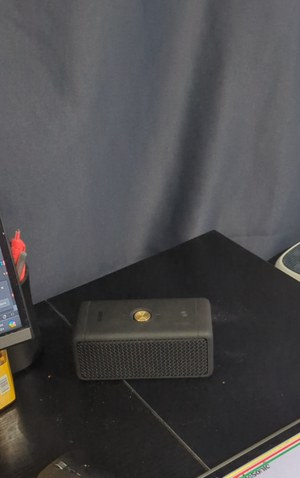
\includegraphics[width=0.31\linewidth]{ex_align_raw.jpg}\hfill
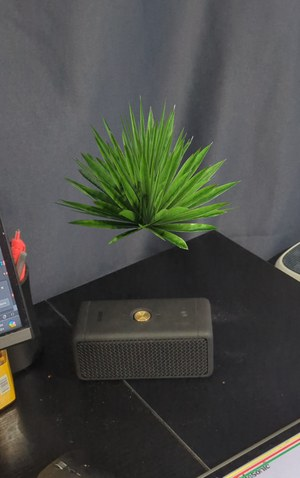
\includegraphics[width=0.31\linewidth]{ex_align_ar.jpg}\hfill
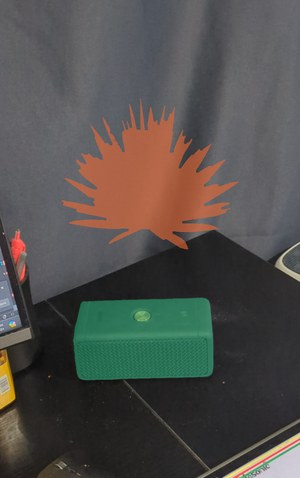
\includegraphics[width=0.31\linewidth]{ex_align_masks.jpg}
\caption{Par benigno do dataset de manipulação ($A=0$, $S=1$, $I=1$, logo $M=0$). Esquerda: $\Ir$.
Centro: $\Ia$, com uma planta virtual acima da caixa de som. Direita: a medida geométrica de
alinhamento (Seção~\ref{sec:hipoteses}): objeto detectado a partir do nome dado pelo Qwen3-VL-4B, em
verde, e conteúdo extraído pela diferença entre as imagens, em laranja. A separação de 142 pixels indica
$A=0$, mas o VLM havia respondido que o conteúdo estava alinhado.}
\label{fig:exemplo}
\end{figure}

% =====================================================================================================
\section{Metodologia}
\label{sec:metodo}

\subsection{Reimplementação e validação}
\label{sec:reconstrucao}
O repositório de Xiu \emph{et al.} traz o dataset e dois notebooks de demonstração com GPT-4o, mas não o
código que produz os resultados publicados. Faltam as linhas de base, as métricas e a geração das
máscaras $m_c$, e os notebooks divergem da descrição publicada em pontos que afetam o resultado (o de obstrução, por
exemplo, sorteia $\alpha$ entre 0,175 e 0,225 a cada imagem). Reimplementamos o pipeline a partir da
descrição publicada, com os prompts transcritos literalmente. Usamos o Grounding DINO aberto no lugar da
versão~1.5, disponível só por API.

Onde a descrição é omissa, tomamos decisões explícitas. A máscara $m_c$ é obtida comparando as duas
fotografias pixel a pixel: como $\Ir$ e $\Ia$ são capturadas do mesmo ponto de vista, os pixels em que
algum canal de cor difere mais de 30 níveis (numa escala de 0 a 255) pertencem ao conteúdo virtual e
recebem 1, e os demais recebem 0. Uma abertura morfológica remove pixels isolados de ruído, e um
fechamento preenche pequenos buracos. O dataset publica só 32 máscaras de conteúdo, sem indicar a que
pares pertencem; as nossas coincidem com elas (IoU mediano de 0,99). Na manipulação, as respostas do VLM
a cada fator, $\hat A$, $\hat S$ e $\hat I$, são lidas da primeira ocorrência de ``yes'' ou ``no'' nas
respostas 3, 4 e 5. O código guarda a resposta bruta do VLM, de modo que regras de decisão e métricas são
recalculadas sem consultar os modelos de novo.

Para validar a reimplementação, comparamos os métodos que não dependem do VLM e o mesmo VLM usado por Xiu \emph{et al.}
com os números publicados. O \emph{prior knowledge} acerta 93,8\% dos pares de obstrução, contra 93,1\%
publicados, e saliência e Canny ficam perto do acaso, como no original; isso confirma detector,
segmentador, $m_c$ e Eq.~\eqref{eq:obs}. Com o LLaVA-Next-8B, o ViDDAR tem 88,2\% contra 89,2\%, e o
end-to-end, 51,3\% contra 55,2\%. Na manipulação, o LLaVA tem 38,6\% de acurácia, 37,0\% de precisão e
84,1\% de recall, contra 43,0\%, 39,8\% e 95,4\% publicados: o padrão é o mesmo (recall alto e precisão
baixa), com diferenças atribuíveis à quantização em 4 bits, à resolução e à decodificação, que diferem
das usadas via API, e a termos uma única execução. Essa é a única comparação direta com os números
publicados; daqui em diante, o objeto de estudo são os cinco VLMs abertos.

\subsection{Modelos e execução}
Avaliamos cinco VLMs abertos de três famílias: Qwen3-VL-2B, Qwen3-VL-4B e Qwen3-VL-8B
(Instruct)~\cite{qwen3vl}, que mostram o efeito do tamanho dentro de uma família; LLaVA-Next-8B~\cite{llava},
o modelo aberto usado por Xiu \emph{et al.}; e Gemma~4 12B~\cite{gemma4}. Todos rodam localmente numa
GPU NVIDIA RTX 3060 de 12~GB: os dois menores em bf16 e os três maiores quantizados em 4 bits
(NF4~\cite{qlora}). A decodificação é determinística (greedy), as imagens são reduzidas a no máximo 1
megapixel e passadas na ordem $\Ir$, $\Ia$, e a resposta é limitada a 768 tokens. Na obstrução, o VLM
leva de 1 a 3~s por par, e a geometria, 0,8~s; na manipulação, o questionário leva de 13 a 23~s por par.

\subsection{Dados}
O dataset de obstrução tem 306 pares de 23 classes de objeto-chave (placas, extintores, tomadas, facas,
entre outras), dos quais 145 são ataques. O de manipulação tem 114 pares, com rótulos de $A$, $S$, $I$ e
$M$ que satisfazem a Eq.~\eqref{eq:man} (Tabela~\ref{tab:composicao}). Os pares benignos foram
construídos tornando falso um ou dois fatores, e quase todos têm dois fatores verdadeiros. Para acertar
um par benigno, o modelo precisa responder ``não'' exatamente ao fator que falha; um modelo que responde
``sim'' a tudo acusa ataque em todos eles. Há também poucos pares que testam a rejeição de $I$: só 11.

\begin{table}[!t]
\renewcommand{\arraystretch}{1.05}
\caption{Composição do dataset de manipulação pelos rótulos dos fatores}
\label{tab:composicao}
\centering
\footnotesize
\begin{tabular}{cccL{3.5cm}c}
\toprule
$A$ & $S$ & $I$ & Par & Pares \\
\midrule
1 & 1 & 1 & ataque ($M=1$) & 44 \\
0 & 1 & 1 & benigno: desalinhado & 32 \\
1 & 0 & 1 & benigno: textura artificial & 25 \\
1 & 1 & 0 & benigno: não sugere nada falso & 11 \\
0 & 0 & 1 & benigno: desalinhado e artificial & 2 \\
\bottomrule
\end{tabular}
\end{table}

\subsection{Convenções, métricas e testes}
\label{sec:metricas}
Usamos a seguinte convenção nas duas tarefas. A classe positiva é o \textbf{ataque}; um par sem ataque é
\textbf{benigno}. O detector \textbf{dispara} quando acusa ataque. Um \textbf{falso positivo} (FP) é
disparar num par benigno, e um \textbf{falso negativo} (FN) é não disparar num ataque. Na manipulação,
responder ``sim'' a um fator afirma uma condição a favor do ataque; por isso, \emph{um viés de ``sim''
produz falsos positivos}, e um viés de ``não'', falsos negativos.

Reportamos acurácia, precisão e recall, as métricas usadas por Xiu \emph{et al.}, e acrescentamos a taxa
de falsos positivos (FPR, fração dos benignos em que o detector dispara) e a de falsos negativos (FNR,
fração dos ataques perdidos, igual a $1-$recall). Os intervalos de 95\% são de Wilson~\cite{wilson}. Duas
execuções são comparadas nos mesmos pares pelo teste exato de McNemar~\cite{mcnemar1947,dietterich1998},
que usa só os pares em que exatamente uma delas acerta; uma diferença só conta com $p<0{,}05$. Na
manipulação, cada execução é comparada também com o detector trivial, que nunca dispara.

Na obstrução, o objeto-chave conta como \textbf{reconhecido} quando a máscara recortada a partir do nome
dado pelo VLM tem IoU $\geq 0{,}5$ com a máscara verdadeira do objeto. Na manipulação, medimos se a
resposta do VLM sobre cada fator $F\in\{A,S,I\}$ depende da imagem pelo índice de Youden~\cite{youden1950}:
\begin{equation}
J_F = P(\hat F=\text{sim}\mid F=1) - P(\hat F=\text{sim}\mid F=0).
\label{eq:youden}
\end{equation}
$J_F$ é a diferença entre a taxa de ``sim'' quando o fator é verdadeiro e quando é falso. Um modelo que
responde ``sim'' sempre, ou ao acaso, tem $J_F=0$, por mais que acerte nos pares em que o fator é
verdadeiro; um juiz perfeito tem $J_F=1$; e $J_F<0$ indica que o modelo diz ``sim'' mais vezes quando o
fator é falso. Ao contrário da acurácia por fator, $J_F$ não premia o viés para o rótulo majoritário.

\subsection{Atribuição de erros}
\label{sec:atrib}
\textbf{Obstrução.} Cada erro do pipeline é atribuído à primeira etapa que falhou: \emph{nada
detectado}, quando o Grounding DINO não encontra o nome; \emph{objeto errado}, quando a máscara
recortada tem IoU $<0{,}5$ com a verdadeira, isto é, o VLM nomeou outro objeto ou o detector achou outro;
e \emph{limiar}, quando o objeto certo foi recortado, mas a fração coberta ficou do lado errado de
$\alpha$. Para separar o que é culpa do VLM do que vem depois dele, olhamos o \emph{prior knowledge} na
mesma amostra. Como ele recebe o nome verdadeiro, se ele acerta, o erro foi introduzido pelo nome que o
VLM deu; se ele também erra, o problema está na detecção, na segmentação, no limiar ou no rótulo.

\textbf{Manipulação.} Como o dataset rotula os três fatores, cada erro recebe uma causa, nesta ordem:
\emph{ilegível}, quando a decisão ou alguma resposta 3--5 não pôde ser interpretada (conta como erro e
nunca é descartada); \emph{conclusão}, quando a resposta 6 contradiz o que as respostas 3--5 implicam
(por exemplo, ``não'' a $I$ seguido de ``sim'' na conclusão); e \emph{percepção}, quando a conclusão segue
as respostas e o erro está nos fatores. Num falso positivo por percepção, o modelo disse ``sim'' aos
fatores cujo rótulo é 0; num falso negativo, disse ``não'' a algum fator verdadeiro. Cada causa é contada
sobre os pares em que pode ocorrer: aceitar um $A$ falso, por exemplo, só pode acontecer nos 32 pares
cujo único fator falso é $A$.

\textbf{Oráculo contrafactual.} Para estimar quanto do erro cada fator explica, trocamos a resposta do
VLM sobre um fator pelo rótulo verdadeiro, mantemos as outras duas e recalculamos
$\hat A\wedge\hat S\wedge\hat I$, sem nova consulta ao modelo. A variação de FPR e FNR é o ganho máximo
de qualquer intervenção que corrija só aquele fator.

\subsection{Hipóteses e intervenções na manipulação}
\label{sec:hipoteses}
A literatura da Seção~\ref{sec:rel} sugere três origens para os erros da manipulação, e cada uma deu
origem a uma intervenção (Fig.~\ref{fig:prompts}). As variantes foram escritas a partir do prompt e das
definições de Xiu \emph{et al.}, e não dos pares em que os modelos erraram, e foram congeladas antes das
execuções completas. O prompt original é a variante \vpaper\ (P).
\begin{itemize}
\item \textbf{O prompt induz o ``sim''} (variante \vneutral, N). O prompt afirma que $\Ia$ foi criada
  ``adicionando conteúdo virtual'' e pede ao modelo que ``pense criativamente'' antes de negar $I$, como
  nas premissas embutidas que levam LLMs a concordar~\cite{sharma2024,pope}. A variante diz que $\Ia$
  ``pode conter'' conteúdo virtual e retira a instrução. Se a hipótese vale, a FPR cai.
\item \textbf{A conclusão ignora as próprias respostas} (variante \vpd, PD). Como o raciocínio pode não
  determinar a resposta final~\cite{turpin2023}, a pergunta 6 pode contradizer as respostas 3--5, e
  responder tudo numa chamada pode fazer um ``sim'' puxar os outros. A variante faz uma chamada para o
  conteúdo e o objeto e uma chamada por fator, e a decisão $\hat A\wedge\hat S\wedge\hat I$ é calculada
  em código~\cite{khot2023}. Para separar os dois efeitos, aplicamos a mesma regra às respostas 3--5 do
  questionário original.
\item \textbf{O VLM julga mal o alinhamento} (medida geométrica). O fator $A$ é o mais geométrico dos
  três, e testamos se uma medida em pixels o julga melhor. Reaproveitamos os componentes da obstrução: o
  nome do objeto dado pelo VLM vai para o Grounding DINO e o SAM, que produzem $m_k$, e $m_c$ vem da
  diferença entre as imagens (Fig.~\ref{fig:exemplo}). A medida é a menor distância entre as duas
  máscaras, dividida pelo maior lado da caixa do conteúdo, e $\Ageo=1$ quando ela fica abaixo de um
  limiar escolhido por validação cruzada estratificada em 5 partições. A \textbf{decisão híbrida} combina
  o alinhamento medido pela geometria com os julgamentos do VLM sobre estilo e informação:
  $\Ageo\wedge\hat S\wedge\hat I$.
\end{itemize}

\begin{figure*}[!t]
\centering
\fbox{\begin{minipage}[t]{0.56\textwidth}\scriptsize
\textsf{\textbf{Prompt original (P), uma chamada com $\Ir$ e $\Ia$}}\\[2pt]\ttfamily\raggedright
Here are two images. The first one is a raw image, and the second one is an augmented image,
\textbf{created by adding some virtual content to the space.}\\
Please answer the following questions:\\
1. What is the virtual content in the augmented image?\\
2. What 'key object' is interacting with the virtual content? Avoid general terms like 'table surface'
or 'environment.'\\
3. Is the virtual content accurately aligned to the object, without a significant gap? Answer yes or
no, then explain why.\\
4. Does the virtual content have a relatively high-quality yet reasonable texture that blends it into
the real world? Answer yes or no, then explain why.\\
5. Do you think the interaction will make users believe the 'key object' has some false functionality
or information it does not have, or lose some true functionality or information it actually has?
\textbf{Think creatively, only say no if the combination has no specific semantic relation.} Answer yes
or no, then explain why.\\
6. If you answered 'yes' in all questions 3, 4, and 5, you must say 'yes.' Otherwise, you say 'no.'
\end{minipage}}\hfill
\fbox{\begin{minipage}[t]{0.40\textwidth}\scriptsize
\textsf{\textbf{Variante neutra (N)}: os dois trechos em negrito mudam}\\[2pt]\ttfamily\raggedright
... augmented image, which may contain virtual content added to the space.\\
(5. sem a frase ``Think creatively...'')\\[4pt]
\textsf{\textbf{Variante decomposta (PD): quatro chamadas}}\\[2pt]
Chamada 1: o preâmbulo de P e ``1. What is the virtual content...? 2. What 'key object'...?'', cada
resposta com até 4 palavras.\\[2pt]
Chamadas 2--4, uma por fator, com o preâmbulo de P e:\\
The virtual content is: \{content\}. The key object interacting with it is: \{key\_obj\}.\\
<pergunta 3, 4 ou 5 de P> Start your answer with yes or no, then explain why.\\[2pt]
Decisão: $\hat A\wedge\hat S\wedge\hat I$, calculada em código.\\[4pt]
\textsf{\textbf{Variante com definição (Seção~\ref{sec:res-hip})}}\\[2pt]
Pergunta 5 precedida da definição de $I$ de Xiu \emph{et al.}: ``Information misrepresentation means that the
combination [...] causes users to misunderstand the scene [...]. Consider a user who takes the virtual
content as part of the real world.''
\end{minipage}}
\caption{Prompts da manipulação. À esquerda, o questionário de Xiu \emph{et al.}, transcrito
literalmente; à direita, o que muda em cada variante. As variantes foram derivadas do texto e das
definições originais, e não dos erros observados.}
\label{fig:prompts}
\end{figure*}

% =====================================================================================================
\section{Resultados: obstrução}
\label{sec:res-obs}

\begin{table}[!t]
\renewcommand{\arraystretch}{1.05}
\caption{Detecção de obstrução nos 306 pares (145 ataques), em \%, com $\alpha=0{,}25$. Em negrito, o
melhor valor de cada linha}
\label{tab:obs}
\centering
\footnotesize
\setlength{\tabcolsep}{3.5pt}
\begin{tabular}{lccccc}
\toprule
 & Qwen 2B & Qwen 4B & Qwen 8B & LLaVA & Gemma \\
\midrule
\multicolumn{6}{l}{\textit{ViDDAR (VLM nomeia, geometria decide)}} \\
\quad acurácia & 84,6 & 91,5 & \textbf{91,8} & 88,2 & 90,5 \\
\quad \scriptsize IC 95\% & \scriptsize 80--88 & \scriptsize 88--94 & \scriptsize 88--94 & \scriptsize 84--91 & \scriptsize 87--93 \\
\quad precisão & 90,8 & 95,4 & \textbf{97,6} & 91,6 & 97,5 \\
\quad recall & 75,2 & \textbf{86,2} & 84,8 & 82,8 & 82,1 \\
\quad FPR & 6,8 & 3,7 & \textbf{1,9} & 6,8 & \textbf{1,9} \\
\quad objeto reconhecido & 72,5 & \textbf{89,9} & 85,0 & 76,1 & 88,6 \\
\midrule
\multicolumn{6}{l}{\textit{End-to-end (VLM decide)}} \\
\quad acurácia & 45,1 & 72,9 & 73,5 & 51,3 & \textbf{81,7} \\
\quad recall & 81,4 & 66,9 & \textbf{84,8} & 8,3 & 80,7 \\
\quad FPR & 87,6 & 21,7 & 36,6 & \textbf{9,9} & 17,4 \\
\midrule
\multicolumn{6}{l}{\textit{Demais linhas de base (acurácia)}} \\
\quad underdetailed & 82,7 & \textbf{85,6} & 82,7 & 82,7 & 80,1 \\
\quad greedy & 88,9 & 90,5 & \textbf{92,2} & 87,3 & 90,5 \\
\quad prior knowledge & \multicolumn{5}{c}{93,8 (nome verdadeiro, sem VLM)} \\
\quad saliência / Canny & \multicolumn{5}{c}{52,3 / 49,7 (sem VLM)} \\
\bottomrule
\multicolumn{6}{L{8.2cm}}{\scriptsize Qwen: Qwen3-VL; LLaVA: LLaVA-Next-8B; Gemma: Gemma~4 12B.
Objeto reconhecido: a máscara recortada a partir do nome dado pelo VLM tem IoU $\geq 0{,}5$ com a
verdadeira.}
\end{tabular}
\end{table}

\subsection{Os VLMs abertos sustentam o detector de obstrução}
A Tabela~\ref{tab:obs} responde à QP1 para a obstrução. Com o pipeline completo, todos os modelos ficam
entre 84,6\% e 91,8\% de acurácia, e três passam de 90\%: Qwen3-VL-4B, Qwen3-VL-8B e Gemma~4, que
empatam entre si no McNemar ($p\geq 0{,}39$). O Qwen3-VL-4B e o Qwen3-VL-8B também não se distinguem do
\emph{prior knowledge} ($p=0{,}065$ e $0{,}15$), que recebe o nome verdadeiro do objeto. Isso significa que,
com esses modelos, escolher o objeto-chave deixa de ser o gargalo: o pipeline erraria quase o mesmo se
soubesse a resposta certa. O Qwen3-VL-2B fica atrás de todos ($p\leq 0{,}001$), e a linha ``objeto
reconhecido'' mostra por quê: ele nomeia o objeto certo em só 72,5\% dos pares, contra 85\% a 90\% dos
três melhores. Na família Qwen, o tamanho ajuda do 2B para o 4B (+6,9 pontos de acurácia), mas não do 4B
para o 8B, que discordam em apenas 13 pares ($p=1{,}0$).

O detector é conservador: a precisão vai de 90,8\% a 97,6\% e a FPR fica abaixo de 7\%, mas o recall fica
entre 75,2\% e 86,2\%. Ou seja, ele raramente acusa uma obstrução inexistente e, quando erra, em geral
deixa passar uma obstrução real. A Seção~\ref{sec:res-obs-erros} mostra que esses dois tipos de erro têm
origens diferentes.

\subsection{Separar reconhecimento e decisão}
A comparação com o end-to-end isola o papel da geometria. Nos cinco modelos, o pipeline com decisão
geométrica supera o end-to-end, com ganhos de 8,8 a 39,5 pontos de acurácia ($p\leq 0{,}001$ em todos).
Quando o VLM decide sozinho se o objeto está coberto, cada modelo revela uma tendência própria, que a
geometria antes neutralizava. O Qwen3-VL-2B responde ``obstruído'' em 259 das 306 amostras (FPR de
87,6\%), e o LLaVA-Next-8B, em apenas 28 (recall de 8,3\%); o Qwen3-VL-8B tende ao ``sim'' (FPR de
36,6\%), e o Qwen3-VL-4B, ao ``não'' (recall de 66,9\%). O Gemma~4 é a exceção: responde ``sim'' em 145
amostras, exatamente o número de ataques, e tem o melhor end-to-end (81,7\%). Como ele não é o melhor em
reconhecer o objeto, sua vantagem está em decidir; uma hipótese, que não testamos, é que o modelo mais
recente e maior do conjunto seja mais bem calibrado em perguntas de sim ou não sobre duas imagens.

\subsection{O prompt define o que é um objeto-chave}
O \emph{underdetailed}, que tira do prompt o papel, a menção a segurança e os exemplos, piora quatro dos
cinco modelos, de 5,5 a 10,4 pontos ($p\leq 0{,}012$). Sem essa orientação, os modelos nomeiam objetos
salientes, mas irrelevantes: ``door'' passa a ser a resposta mais frequente do Gemma~4 (29 vezes) e do
Qwen3-VL-2B (27), e o reconhecimento do Gemma~4 cai de 88,6\% para 62,1\%. O papel e os exemplos não
ensinam o modelo a ver melhor; eles dizem \emph{que tipo} de objeto conta como importante. O
\emph{greedy} empata com o pipeline padrão em quase todos os modelos. A exceção é o Qwen3-VL-2B (de 84,6\%
para 88,9\%, $p=0{,}007$): para o modelo que mais erra o objeto, listar vários candidatos compensa a
escolha errada de um só.

\subsection{De onde vêm os erros}
\label{sec:res-obs-erros}

\begin{table}[!t]
\renewcommand{\arraystretch}{1.05}
\caption{Obstrução: erros do pipeline por etapa (Seção~\ref{sec:atrib}). Entre parênteses, quantas
dessas amostras o \emph{prior knowledge}, que recebe o nome verdadeiro, também erra}
\label{tab:obs-causas}
\centering
\footnotesize
\setlength{\tabcolsep}{3.2pt}
\begin{tabular}{llccccc}
\toprule
Erro & Etapa & Qwen 2B & 4B & 8B & LLaVA & Gemma \\
\midrule
FP & objeto errado & 11 (0) & 6 (0) & 3 (0) & 11 (0) & 3 (0) \\
\midrule
\multirow{3}{*}{FN} & nada detectado & 3 (0) & 0 & 0 & 0 & 0 \\
 & objeto errado & 17 (2) & 5 (3) & 7 (2) & 15 (6) & 12 (4) \\
 & limiar & 16 (14) & 15 (14) & 15 (14) & 10 (9) & 14 (13) \\
\bottomrule
\multicolumn{7}{l}{\scriptsize De 161 pares benignos (FP) e 145 ataques (FN). O \emph{prior} tem 1 FP e 18 FN.}
\end{tabular}
\end{table}

A Tabela~\ref{tab:obs-causas} responde à QP2 para a obstrução, e os dois tipos de erro contam histórias
distintas.

\textbf{Falsos positivos: qual objeto importa.} Todos os falsos positivos são de reconhecimento, e o
\emph{prior knowledge} acerta todas essas amostras (o zero entre parênteses). Em cada caso, o VLM nomeia
um objeto diferente do anotado, e o conteúdo virtual cobre esse outro objeto. Os casos se concentram em
cenas com mais de um objeto plausível (Fig.~\ref{fig:obs-fp}): diante de uma placa de advertência
pregada numa porta, quatro modelos nomeiam a porta (``black door with sign''); diante de uma panela
fervendo, quatro nomeiam o queimador ou o fogão (``glowing red burner'', ``black stove''). Fora dessas
classes e de tomadas, o Qwen3-VL-4B, o Qwen3-VL-8B e o Gemma~4 somam só 2 falsos positivos. O
Qwen3-VL-2B tem um modo de falha próprio: em 36 das 306 imagens ele responde ``red box'', copiando o
exemplo do prompt, e 5 dos seus 11 falsos positivos vêm disso (Fig.~\ref{fig:redbox}). Os falsos
positivos da obstrução, portanto, não vêm de percepção visual nem da geometria, e sim de uma escolha que
o prompt não especifica: em cenas ambíguas, o VLM escolhe um candidato razoável diferente do anotado.

\begin{figure}[!t]
\centering
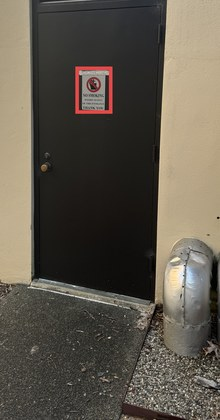
\includegraphics[height=2.75cm]{ex_fp_warning-sign_002_raw.jpg}\hspace{1pt}%
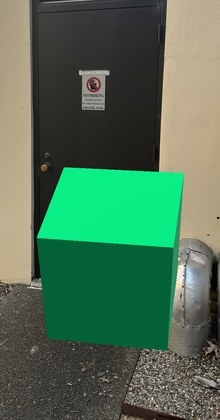
\includegraphics[height=2.75cm]{ex_fp_warning-sign_002_ar.jpg}\hfill
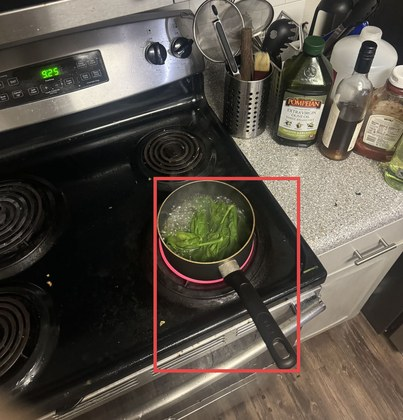
\includegraphics[height=2.75cm]{ex_fp_boiling-pot_010_raw.jpg}\hspace{1pt}%
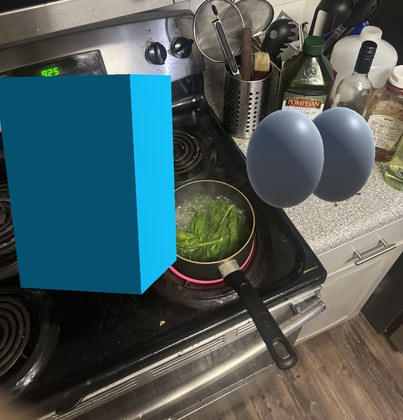
\includegraphics[height=2.75cm]{ex_fp_boiling-pot_010_ar.jpg}
\caption{Dois pares benignos de obstrução em que quatro dos cinco VLMs disparam. Em cada par, à
esquerda, $\Ir$ com o objeto-chave anotado (contorno vermelho) e, à direita, $\Ia$. Esquerda: a placa de
advertência; os modelos nomeiam a porta, coberta em 41\% pelo cubo virtual. Direita: a panela; os modelos
nomeiam o queimador ou o fogão, cobertos em 25\% a 47\%.}
\label{fig:obs-fp}
\end{figure}

\begin{figure}[!t]
\centering
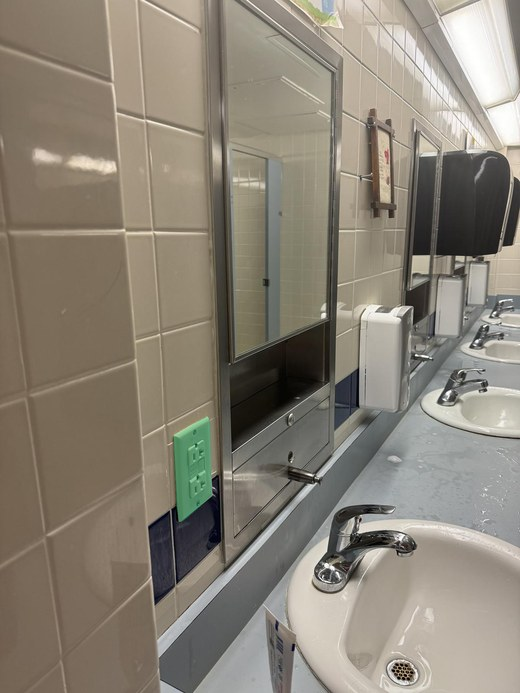
\includegraphics[height=3.6cm]{ex_obs_key.jpg}\hspace{4pt}%
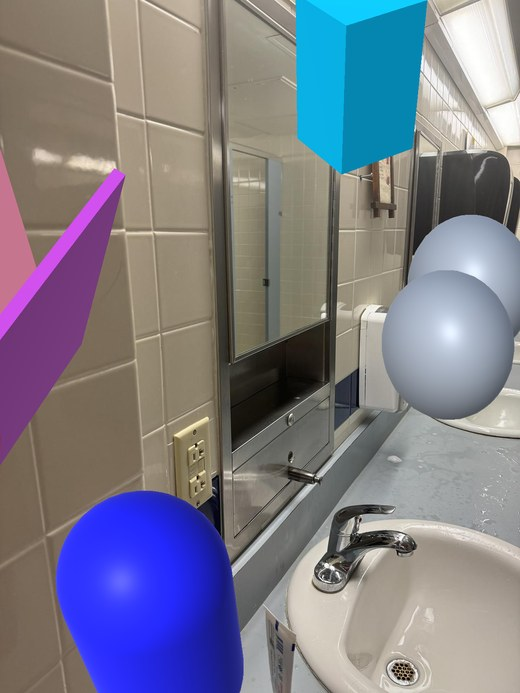
\includegraphics[height=3.6cm]{ex_obs_ar.jpg}
% VERIFICAR: o objeto encontrado pelo Grounding DINO foi inferido pela imagem; conferir a caixa em
% results/obstruction/qwen3-vl-2b/viddar/predictions.csv (par electrical-outlet_004).
\caption{Falso positivo do Qwen3-VL-2B por cópia do prompt. Esquerda: $\Ir$, com o objeto-chave anotado
(a tomada) em verde. Direita: $\Ia$. O VLM respondeu ``red box'', o exemplo do prompt. O Grounding DINO
procurou esse nome em $\Ir$ e encontrou o objeto avermelhado mais próximo da descrição, o quadro de
moldura marrom na parede, que está 45\% coberto pelo cubo ciano virtual. Pela Eq.~\eqref{eq:obs}, o
pipeline acusou obstrução de um objeto que não era o objeto-chave; a tomada não está coberta.}
\label{fig:redbox}
\end{figure}

\textbf{Falsos negativos: cobertura logo abaixo de $\alpha$.} Os falsos negativos são o erro dominante
(FNR de 13,8\% a 24,8\%) e, ao contrário dos falsos positivos, em geral não dependem do VLM. De 10 a 16
por modelo são de limiar: o objeto certo foi recortado, mas a fração coberta ficou entre 0,06 e 0,249,
com mediana de cerca de 0,21, logo abaixo de $\alpha=0{,}25$. O \emph{prior knowledge} erra quase todos
eles, e 7 se repetem nos cinco modelos. Coerentemente, a acurácia de todos os modelos, e também a do
\emph{prior}, é máxima com $\alpha=0{,}20$, de 1,0 a 2,0 pontos acima da obtida com $0{,}25$. A
explicação provável é que as nossas máscaras $m_c$ sejam um pouco menores que as usadas na rotulagem.
Mantivemos $\alpha=0{,}25$, porque escolher o limiar no conjunto de teste seria otimista, e a ordem dos
modelos não muda com $\alpha$.

% =====================================================================================================
\section{Resultados: manipulação de informação}
\label{sec:res-man}

\begin{table*}[!t]
\renewcommand{\arraystretch}{1.0}
\caption{Detecção de manipulação nos 114 pares (44 ataques), em \%, com o prompt original (P) e as
variantes neutra (N) e decomposta (PD) da Fig.~\ref{fig:prompts}. ``vs.~P'': diferença de acurácia para o
prompt original e $p$ do McNemar. ``vs.~trivial'': comparação, pelo McNemar, com o detector que nunca
dispara (61,4\%); n.s. = sem diferença significativa. $J$: índice de Youden de cada fator
(Eq.~\ref{eq:youden}), 0 quando a resposta não depende da imagem}
\label{tab:man}
\centering
\footnotesize
\setlength{\tabcolsep}{4.2pt}
\begin{tabular}{llcccccccccc}
\toprule
Modelo & Variante & Acurácia & Precisão & Recall & FPR & FNR & vs.~P ($p$) & vs.~trivial & $J_A$ & $J_S$ & $J_I$ \\
\midrule
\multirow{3}{*}{Qwen3-VL-2B}
 & P  & 38,6 & 38,2 & 95,5 & 97,1 & 4,5 & -- & abaixo & $-$0,03 & $-$0,02 & 0,00 \\
 & N  & 48,2 & 42,7 & 93,2 & 78,6 & 6,8 & +9,6 (0,019) & n.s. & $-$0,03 & $-$0,01 & 0,00 \\
 & PD & 37,7 & 37,4 & 90,9 & 95,7 & 9,1 & $-$0,9 (n.s.) & abaixo & $-$0,03 & 0,07 & 0,00 \\
\midrule
\multirow{3}{*}{Qwen3-VL-4B}
 & P  & 61,4 & 50,0 & 6,8 & 4,3 & 93,2 & -- & n.s. & 0,09 & 0,31 & $-$0,30 \\
 & N  & 61,4 & -- & 0,0 & 0,0 & 100 & 0,0 (n.s.) & n.s. & 0,28 & 0,41 & $-$0,20 \\
 & PD & 73,7 & 93,8 & 34,1 & 1,4 & 65,9 & +12,3 (0,003) & \textbf{acima} & 0,25 & 0,22 & $-$0,01 \\
\midrule
\multirow{3}{*}{Qwen3-VL-8B}
 & P  & 37,7 & 38,1 & 97,7 & 100 & 2,3 & -- & abaixo & 0,48 & 0,25 & $-$0,01 \\
 & N  & 60,5 & 49,4 & 90,9 & 58,6 & 9,1 & +22,8 ($<$0,001) & n.s. & 0,48 & 0,22 & 0,08 \\
 & PD & 69,3 & 61,5 & 54,5 & 21,4 & 45,5 & +31,6 ($<$0,001) & n.s. & 0,32 & 0,50 & $-$0,09 \\
\midrule
\multirow{3}{*}{LLaVA-Next-8B}
 & P  & 38,6 & 37,0 & 84,1 & 90,0 & 15,9 & -- & abaixo & $-$0,13 & $-$0,02 & 0,00 \\
 & N  & 53,5 & 42,6 & 59,1 & 50,0 & 40,9 & +14,9 (0,014) & n.s. & 0,05 & $-$0,03 & 0,00 \\
 & PD & 63,2 & 55,0 & 25,0 & 12,9 & 75,0 & +24,6 (0,003) & n.s. & 0,05 & $-$0,06 & 0,00 \\
\midrule
\multirow{3}{*}{Gemma 4 12B}
 & P  & 55,3 & 46,2 & 95,5 & 70,0 & 4,5 & -- & n.s. & 0,20 & 0,16 & 0,25 \\
 & N  & 59,6 & 48,2 & 61,4 & 41,4 & 38,6 & +4,4 (n.s.) & n.s. & 0,24 & 0,31 & 0,18 \\
 & PD & 61,4 & -- & 0,0 & 0,0 & 100 & +6,1 (n.s.) & n.s. & 0,35 & 0,00 & 0,21 \\
\bottomrule
\multicolumn{12}{l}{\scriptsize Precisão indefinida (--) quando o modelo nunca dispara. O $J_I$ usa só os 11 pares com $I=0$ e é pouco preciso.}
\end{tabular}
\end{table*}

\begin{figure*}[!t]
\centering
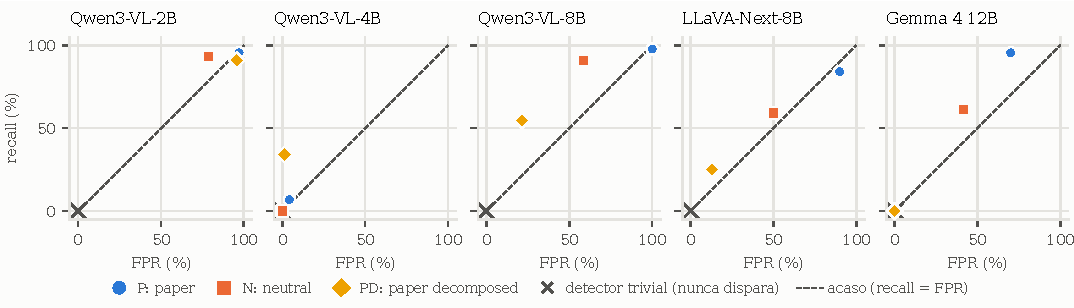
\includegraphics[width=\textwidth]{fig_op.pdf}
\caption{Recall contra FPR de cada variante na manipulação. O canto superior esquerdo é o ideal; a
diagonal tracejada é o desempenho de um detector que ignora as imagens e dispara ao acaso, e o $\times$,
na origem, é o detector trivial que nunca dispara. Com o prompt original (P), quatro modelos ficam
sobre a diagonal, e só o Gemma~4 fica acima dela. As variantes, em geral, deslizam o ponto ao longo da
diagonal, trocando falsos positivos por falsos negativos; só as decompostas do Qwen3-VL-4B e do
Qwen3-VL-8B se afastam dela.}
\label{fig:op}
\end{figure*}

\subsection{Nenhum modelo supera o detector trivial}
A Tabela~\ref{tab:man} e a Fig.~\ref{fig:op} respondem à QP1 para a manipulação, e a resposta é
negativa. Com o prompt original, nenhum modelo acerta significativamente mais que o detector que nunca
dispara. Três deles ficam significativamente \emph{abaixo}: o Qwen3-VL-2B, o Qwen3-VL-8B e o
LLaVA-Next-8B disparam em 90\% a 100\% dos pares benignos e, por isso, erram quase todos os 70. O
Qwen3-VL-4B tem exatamente a acurácia do detector trivial pelo motivo oposto: quase nunca dispara
(recall de 6,8\%). O Gemma~4 fica no meio (55,3\%).

A Fig.~\ref{fig:op} mostra o que a acurácia esconde. Quatro dos cinco modelos ficam sobre a diagonal:
disparam nos ataques e nos pares benignos na mesma proporção, como um detector que não olha as imagens.
Só o Gemma~4 fica acima dela, com recall de 95,5\% e FPR de 70\%, um sinal fraco de discriminação. Como há
mais pares benignos que ataques, qualquer deslocamento para o ``não'' aumenta a acurácia sem que o modelo
discrimine melhor; por isso, nas variantes, a comparação com o detector trivial é mais informativa que o
ganho de acurácia. O LLaVA-Next-8B decomposto, por exemplo, sobe de 38,6\% para 63,2\% de acurácia, mas o
recall cai de 84\% para 25\%: ele passou a perder três de cada quatro ataques. Das 15 configurações, só
uma supera o detector trivial: o Qwen3-VL-4B decomposto (73,7\%), que detecta 15 dos 44 ataques com um
único alarme falso (precisão de 93,8\%). O Qwen3-VL-8B decomposto é o detector mais equilibrado (recall de
54,5\% e FPR de 21,4\%), mas não se distingue do trivial ($p=0{,}20$).

\subsection{As causas dos erros}
\label{sec:res-man-causas}

\begin{table}[!t]
\renewcommand{\arraystretch}{1.05}
\caption{Manipulação: causas dos erros com o prompt original (Seção~\ref{sec:atrib}). Cada célula é o
número de erros sobre o número de pares em que a causa pode ocorrer}
\label{tab:causas}
\centering
\footnotesize
\setlength{\tabcolsep}{2.6pt}
\begin{tabular}{llccccc}
\toprule
 & Causa & Qwen 2B & 4B & 8B & LLaVA & Gemma \\
\midrule
\multirow{5}{*}{FP} & conclusão & 68/70 & 0/70 & 44/70 & 0/70 & 0/70 \\
 & aceitou $A$ falso & 0/32 & 2/32 & 10/32 & 31/32 & 22/32 \\
 & aceitou $S$ falso & 0/25 & 1/25 & 11/25 & 22/25 & 18/25 \\
 & aceitou $I$ falso & 0/11 & 0/11 & 5/11 & 8/11 & 7/11 \\
 & aceitou $A$ e $S$ falsos & 0/2 & 0/2 & 0/2 & 2/2 & 2/2 \\
\midrule
\multirow{3}{*}{FN} & rejeitou $I$ verdadeiro & 0/44 & 38/44 & 0/44 & 0/44 & 0/44 \\
 & rejeitou $A$ e/ou $S$ & 0/44 & 3/44 & 1/44 & 7/44 & 1/44 \\
 & ilegível ou conclusão & 2/44 & 0/44 & 0/44 & 0/44 & 1/44 \\
\midrule
\multicolumn{2}{l}{Total FP / FN} & 68 / 2 & 3 / 41 & 70 / 1 & 63 / 7 & 49 / 2 \\
\bottomrule
\end{tabular}
\end{table}

A Tabela~\ref{tab:causas} responde à QP2 para a manipulação: não há uma causa comum, e cada modelo tem a
sua.

\textbf{Conclusão que contradiz as respostas (Qwen3-VL-2B e Qwen3-VL-8B).} No Qwen3-VL-2B, 68 dos 70
falsos positivos são de conclusão: ele responde ``não'' a $I$ em todos os pares, o que deveria levar a
``não'' na pergunta 6, e mesmo assim conclui ``sim'' em 96\% deles, muitas vezes afirmando ter dito
``sim'' às perguntas 3 a 5. O Qwen3-VL-8B faz o mesmo de forma mais clara: responde ``Yes.'' na pergunta
6 em 113 dos 114 pares, inclusive depois de negar o alinhamento:
\vlmbox{Qwen3-VL-8B, par benigno com $A=0$, prompt original}{3. No. The virtual plant is positioned
floating in the air directly above the hard drive, with a clear gap [...]\\ 6. Yes.}

\textbf{Aceitação de alinhamento e estilo ruins (LLaVA-Next-8B e Gemma~4).} Nesses dois modelos, a
conclusão segue as respostas, mas as respostas aceitam quase tudo: o LLaVA aceita o alinhamento em 31 dos
32 pares desalinhados, e o Gemma~4, em 22; o estilo, em 22 e 18 dos 25 pares com textura artificial. O
LLaVA chega a descrever o desalinhamento e, logo depois, negá-lo:
\vlmbox{LLaVA-Next-8B, par benigno com $A=0$, prompt original}{1. [...] a cup of coffee with a saucer,
floating above the fan.\\ 3. Yes, the virtual content is accurately aligned to the fan without a
significant gap.}

\textbf{Leitura restritiva de $I$ (Qwen3-VL-4B).} O Qwen3-VL-4B quase não aceita fatores falsos (3 falsos
positivos), mas rejeita $I$ em 38 dos 44 ataques. Ele identifica o conteúdo e o objeto, mas entende
``informação falsa'' como algo absurdo e trata adições plausíveis como inofensivas: uma cesta virtual
num patinete seria ``um acessório plausível''. Para o método de referência é o contrário: é a
plausibilidade que faz o usuário acreditar que a cesta existe. A FPR baixa desse modelo, portanto, não é
mérito, mas consequência de rejeitar $I$.

\textbf{Os modelos percebem os fatores?} As colunas $J$ da Tabela~\ref{tab:man} medem se a resposta a
cada fator muda conforme o fator é verdadeiro ou falso. No Qwen3-VL-2B e no LLaVA-Next-8B, $|J|\leq 0{,}13$
em todos os fatores e variantes: esses modelos respondem de forma quase igual a pares alinhados e
desalinhados, realistas e artificiais, e as variantes só mudam a frequência com que dizem ``sim''. Na
família Qwen, o tamanho melhora a percepção do alinhamento: $J_A$ vai de $-0{,}03$ no 2B a 0,09 no 4B e
0,48 no 8B. Nenhum modelo, porém, distingue $I$: nas 15 configurações, $J_I$ fica entre $-0{,}30$ e
$0{,}25$, e só o Gemma~4 tem valores positivos em todas, com intervalos largos.

\textbf{Quanto cada fator explica.} O oráculo (Tabela~\ref{tab:oraculo}) mostra que nenhum fator
corrigido sozinho leva a um bom detector, porque a decisão é uma conjunção: um erro num fator só aparece
se os outros dois forem aceitos, e erros num fator ficam escondidos atrás de erros em outro. No
LLaVA-Next-8B e no Gemma~4, corrigir $A$ dá a maior queda de FPR (de 90,0\% para 42,9\% e de 72,9\% para
37,1\%), porque o desalinhamento é o tipo de par benigno mais comum; só corrigindo $A$ e $S$ juntos a FPR
cairia para 15,7\% e 11,4\%. No Qwen3-VL-4B, corrigir $I$ reduz a FNR de 93,2\% para 6,8\%, mas a FPR sobe
de 4,3\% para 47,1\%: os 65\% de pares desalinhados que o modelo aceita deixam de ser barrados pela
rejeição de $I$. No Qwen3-VL-2B, corrigir $A$ ou $S$ não muda nada, porque ele nega $I$ sempre.

\begin{table}[!t]
\renewcommand{\arraystretch}{1.05}
\caption{Manipulação: oráculo contrafactual com o prompt original. FPR / FNR (\%) da regra
$\hat A\wedge\hat S\wedge\hat I$ quando a resposta do VLM sobre o fator indicado é trocada pelo rótulo
verdadeiro}
\label{tab:oraculo}
\centering
\footnotesize
\setlength{\tabcolsep}{2.4pt}
\begin{tabular}{lccccc}
\toprule
 & nenhum & $A$ & $S$ & $I$ & $A$ e $S$ \\
\midrule
Qwen 2B & 0 / 100 & 0 / 100 & 0 / 100 & 84 / 5 & 0 / 100 \\
Qwen 4B & 4 / 93 & 1 / 93 & 3 / 93 & \textbf{47 / 7} & 10 / 86 \\
Qwen 8B & 37 / 5 & 23 / 5 & 21 / 5 & 30 / 5 & 16 / 2 \\
LLaVA & 90 / 16 & \textbf{43} / 16 & 56 / 16 & 79 / 16 & \textbf{16 / 0} \\
Gemma & 73 / 2 & \textbf{37 / 0} & 44 / 2 & 61 / 2 & 11 / 0 \\
\bottomrule
\multicolumn{6}{L{8.2cm}}{\scriptsize A coluna ``nenhum'' usa a regra sobre as respostas 3--5, e não a
pergunta 6; por isso difere da Tabela~\ref{tab:man} no Qwen 2B e no Qwen 8B.}
\end{tabular}
\end{table}

\subsection{O que as intervenções corrigem}
\label{sec:res-hip}
\textbf{O prompt induz o ``sim'': confirmada nos modelos que disparam demais.} Com a variante neutra, a
FPR cai em todos os modelos que disparavam demais: de 97\% para 79\% no Qwen3-VL-2B, de 100\% para 59\% no
Qwen3-VL-8B, de 90\% para 50\% no LLaVA-Next-8B e de 70\% para 41\% no Gemma~4, e a acurácia sobe com
significância nos três primeiros. O prompt original, portanto, empurra os modelos para o ``sim''. Mas a
queda de falsos positivos só é um ganho real nos modelos que percebem os fatores; nos demais, ela vira
aumento de falsos negativos. No Gemma~4, a FNR sobe de 4,5\% para 38,6\%, e no LLaVA, de 15,9\% para
40,9\%: os pontos da Fig.~\ref{fig:op} deslizam ao longo da diagonal.

\textbf{A conclusão ignora as respostas: confirmada, e é o principal problema do Qwen3-VL-8B.} A variante
decomposta elimina por construção o erro de conclusão e dá os maiores ganhos de acurácia em relação ao
prompt original: +12,3 pontos no Qwen3-VL-4B, +31,6 no Qwen3-VL-8B e +24,6 no LLaVA-Next-8B, este à custa
do recall. No lugar da conclusão, porém, aparece o viés de cada pergunta isolada. O Qwen3-VL-4B e o
Gemma~4 passam a rejeitar o estilo; o Gemma descreve o conteúdo como ``a 2D sticker placed over the
image'' em todos os pares e vira um detector que nunca dispara. O LLaVA passa a rejeitar o alinhamento em
28 dos 44 ataques. A decomposição muda duas coisas ao mesmo tempo, quem decide e quantas perguntas cada
chamada faz. Para isolar a primeira, aplicamos a regra $\hat A\wedge\hat S\wedge\hat I$ às respostas 3--5
do questionário original, sem nova consulta. No Qwen3-VL-8B, cuja resposta 6 concorda com a regra em só
60,5\% dos pares, essa troca leva a acurácia de 37,7\% para 75,4\% (44 pares corrigidos e 1 piorado,
$p<0{,}001$) e a FPR de 100\% para 37,1\%, o melhor resultado com o questionário original, embora ainda
não significativamente acima do detector trivial ($p=0{,}068$). O Qwen3-VL-8B percebe o alinhamento e o
estilo razoavelmente bem, mas ignora as próprias respostas na hora de decidir. No Qwen3-VL-2B, a mesma
troca leva a 61,4\%, que é o próprio detector trivial, porque ele nega $I$ sempre. Nos outros três
modelos, a resposta 6 já concorda com a regra em 88\% a 100\% dos pares.

\textbf{Definir $I$ não ensina o modelo a distinguir $I$.} Uma pergunta natural é se explicar ao modelo o
que é $I$ resolveria a leitura restritiva. Testamos uma terceira variante, com a definição de $I$ dada
por Xiu \emph{et al.} antes da pergunta 5 (Fig.~\ref{fig:prompts}). Se ela funcionasse, o modelo passaria a dizer
``sim'' a $I$ nos ataques e continuaria dizendo ``não'' nos 11 pares em que $I$ é falso, e $J_I$
subiria. Não foi o que aconteceu. No questionário único, os efeitos foram em direções opostas e nenhum
ganho veio de $I$. No modo decomposto, o Qwen3-VL-8B ganhou 6,1 pontos sobre a variante decomposta sem
definição (75,4\% de acurácia, $p=0{,}016$), e os falsos negativos causados por $I$ sumiram (de 7 para
0). Essa configuração chega a superar o detector trivial, mas pelo motivo errado. $J_I$ foi de
$-0{,}09$ para 0,00: o modelo passou a responder ``sim'' a $I$ em \emph{todos} os pares, inclusive nos 11
em que $I$ é falso. Como $I$ é verdadeiro em 103 dos 114 pares, dizer sempre
``sim'' acerta quase sempre. O ganho vem da composição do dataset, e não de uma leitura melhor de $I$, e
o detector se reduz, na prática, a $\hat A\wedge\hat S$.

\textbf{O VLM julga mal o alinhamento: confirmada no fator, não na decisão.} A medida geométrica julga $A$
melhor que o VLM em quatro dos cinco modelos, e o Gemma~4 empata (Tabela~\ref{tab:c2}). Independentemente
do limiar, a distância separa os pares alinhados dos desalinhados com AUC de 0,70 a 0,79. Na decisão,
porém, a decisão híbrida só melhora com significância no LLaVA-Next-8B, e por troca: a FPR cai de 90\%
para 41\%, mas a FNR sobe de 16\% para 57\%. Comparamos o híbrido com a regra
$\hat A\wedge\hat S\wedge\hat I$, e não com a resposta 6, porque só assim a diferença se deve ao $A$
geométrico, e não à troca da conclusão. Um $A$ melhor ajuda pouco porque, de novo, a decisão é uma
conjunção: onde $S$ ou $I$ já barram o ataque, como no Qwen3-VL-2B e no Qwen3-VL-4B, $A$ não muda nada;
onde o VLM aceita tudo, a geometria corta falsos positivos, mas também ataques, porque a própria medida
erra de 20\% a 35\% dos pares. O oráculo já antecipava esse teto: mesmo com $A$ perfeito, a FPR do LLaVA
não cairia abaixo de 43\%.

\begin{table}[!t]
\renewcommand{\arraystretch}{1.05}
\caption{Manipulação: alinhamento geométrico com o prompt original. Acerto no fator $A$ e acurácia da
decisão. A decisão híbrida $\Ageo\wedge\hat S\wedge\hat I$ é comparada com a regra
$\hat A\wedge\hat S\wedge\hat I$ sobre as respostas do próprio VLM, o que isola o efeito do $A$
geométrico}
\label{tab:c2}
\centering
\footnotesize
\setlength{\tabcolsep}{4pt}
\begin{tabular}{lcccc}
\toprule
 & \multicolumn{2}{c}{Acerto em $A$ (\%)} & \multicolumn{2}{c}{Acurácia da decisão (\%)} \\
\cmidrule(lr){2-3}\cmidrule(lr){4-5}
Modelo & VLM & geometria & $\hat A\wedge\hat S\wedge\hat I$ & híbrida \\
\midrule
Qwen3-VL-2B   & 70 & \textbf{79} & 61,4 & 61,4 \\
Qwen3-VL-4B   & 62 & \textbf{76} & 61,4 & 61,4 \\
Qwen3-VL-8B   & 75 & \textbf{80} & 75,4 & 78,1 \\
LLaVA-Next-8B & 60 & \textbf{65} & 38,6 & \textbf{52,6}$^{*}$ \\
Gemma 4 12B   & 74 & 73 & 54,4 & 59,6 \\
\bottomrule
\multicolumn{5}{L{7.4cm}}{\scriptsize $^{*}$Única diferença significativa entre as duas decisões
(McNemar, $p=0{,}036$; nas demais, $p\geq 0{,}36$).}
\end{tabular}
\end{table}

% =====================================================================================================
\section{Discussão}
\label{sec:disc}

\textbf{O que separa as duas tarefas é quem decide.} Os mesmos VLMs que chegam a cerca de 91\% na
obstrução não superam o detector trivial na manipulação. A diferença não está no tamanho dos modelos nem
na dificuldade visual das cenas, mas no papel do VLM: na obstrução, ele dá uma resposta curta e
localizada (um nome), e uma regra explícita decide; quando decide sozinho, no end-to-end, aparecem os
mesmos vieses de ``sim'' e de ``não'' observados na manipulação. Na manipulação, os melhores resultados
também vieram de tirar a decisão do VLM. Para quem projeta esses detectores com modelos pequenos, a
lição é usar o VLM como fonte de julgamentos simples e verificáveis, e não como juiz da decisão final.

\textbf{Os falsos positivos têm naturezas diferentes nas duas tarefas.} Na obstrução, eles são poucos,
interpretáveis e vêm de ambiguidade semântica: em cenas com mais de um candidato razoável, o VLM escolhe
um diferente do anotado. Corrigi-los exige especificar melhor o que é o objeto-chave, no prompt ou no
rótulo, e não um modelo maior. Na manipulação, os falsos positivos são sistemáticos e vêm de vieses do
modelo, como a concordância com o prompt e a conclusão que ignora as próprias respostas, ou de percepção
fraca dos fatores. Intervenções no prompt e na forma de decidir só os reduzem sem custo nos modelos que
percebem os fatores, como o Qwen3-VL-8B ($J_A=0{,}48$); no LLaVA-Next-8B ($J_A\approx 0$), apenas trocam
falsos positivos por falsos negativos.

\textbf{Escala ajuda, mas não resolve o fator semântico.} Na família Qwen, o modelo maior reconhece
melhor o objeto-chave (do 2B para o 4B) e percebe melhor o alinhamento e o estilo (do 4B para o 8B), mas
esse ganho só aparece na manipulação quando a conclusão sai do VLM. O fator $I$, que distingue um ataque
de um conteúdo apenas bem encaixado, não é medido de forma confiável por nenhum modelo, nem mesmo quando
o prompt traz sua definição. Como referência, o GPT-4o acerta 82,5\% dos pares de manipulação segundo
Xiu \emph{et al.}~\cite{viddar}; nenhum dos VLMs abertos chega a esse nível com o questionário. O dataset também
testa $I$ mal, com só 11 pares em que ele é falso. Um benchmark para essa tarefa deveria equilibrar as
combinações de fatores e reportar FPR, FNR e a comparação com o detector trivial, já que, com mais pares
benignos que ataques, um detector mais conservador ganha acurácia sem discriminar melhor.

% =====================================================================================================
\section{Limitações e trabalhos futuros}
\label{sec:lim}

Os datasets são pequenos (306 e 114 pares), e as conclusões sobre $I$ se apoiam em 11 pares. As variantes
de prompt e a regra $\hat A\wedge\hat S\wedge\hat I$ foram avaliadas nos mesmos dados, sem conjunto de
teste separado; com várias configurações e testes, algum $p<0{,}05$ pode ser acaso, embora as variantes
tenham sido escritas a partir das definições originais, e não dos erros, e todas sejam reportadas. Os VLMs têm de 2 a 12
bilhões de parâmetros, os três maiores rodam em 4 bits, e há uma única execução por configuração, sem
estimativa da variância. A comparação com os resultados publicados usa os números de Xiu \emph{et al.}, sem teste
pareado. As máscaras $m_c$ derivadas da diferença de pixels só valem para pares alinhados pixel a pixel e
provavelmente explicam o $\alpha$ ótimo de 0,20. Na obstrução, a categoria ``objeto errado'' mistura erros
do VLM e do detector, e o \emph{prior knowledge} separa só parte deles. Fatores e decisão são lidos por
regras sobre o texto, com no máximo 2 respostas ilegíveis por execução.

Como próximos passos, propomos validar as configurações escolhidas em dados novos, estimar a variância
com execuções repetidas, construir um conjunto com mais pares benignos em que $I$ é falso, buscar sinais
mensuráveis para o estilo e especificar no prompt como escolher entre objetos-chave concorrentes. Também
interessa avaliar os detectores em cenas menos controladas, com degradação física de objetos e
sobreposições já presentes na imagem, que podem ser tomadas por conteúdo virtual.

% =====================================================================================================
\section{Conclusão}

Avaliamos cinco VLMs abertos, executados localmente, como base de detectores de conteúdo prejudicial em
RA. Na obstrução, o pipeline de referência é robusto à troca do VLM: três modelos passam de 90\% de
acurácia, os poucos falsos positivos vêm da escolha de outro objeto plausível em cenas ambíguas, e os
falsos negativos se concentram logo abaixo do limiar, sem depender do VLM. Na manipulação, com o
questionário original, nenhum modelo supera um detector que nunca dispara. Atribuindo cada erro a uma
causa, mostramos que eles vêm de conclusões que contradizem as próprias respostas, de um viés de ``sim''
induzido pelo prompt e de percepção fraca dos fatores, com uma causa dominante diferente em cada modelo.
As intervenções só reduzem falsos positivos sem perder ataques nos modelos que percebem os fatores, a
medida geométrica julga o alinhamento melhor que os VLMs sem melhorar a decisão, e nenhum modelo distingue
o fator semântico que define o ataque. Nas duas tarefas, o detector funciona melhor quando a decisão
final não fica com o VLM.

\begin{thebibliography}{99}

\bibitem{viddar}
Y.~Xiu, T.~Scargill, and M.~Gorlatova, ``{ViDDAR}: Vision language model-based task-detrimental
content detection for augmented reality,'' \emph{IEEE Trans. Vis. Comput. Graphics}, vol.~31, no.~5,
pp. 3194--3203, 2025, doi: 10.1109/TVCG.2025.3549147.

\bibitem{roesner2014}
F.~Roesner, T.~Kohno, and D.~Molnar, ``Security and privacy for augmented reality systems,''
\emph{Commun. ACM}, vol.~57, no.~4, pp. 88--96, 2014.

\bibitem{arya}
K.~Lebeck, K.~Ruth, T.~Kohno, and F.~Roesner, ``Securing augmented reality output,'' in \emph{Proc.
IEEE Symp. Security Privacy (SP)}, 2017, pp. 320--337.

\bibitem{cheng2023}
K.~Cheng, J.~F. Tian, T.~Kohno, and F.~Roesner, ``Exploring user reactions and mental models towards
perceptual manipulation attacks in mixed reality,'' in \emph{Proc. USENIX Security Symp.}, 2023.

\bibitem{vimsense}
Y.~Xiu and M.~Gorlatova, ``Detecting visual information manipulation attacks in augmented reality: A
multimodal semantic reasoning approach,'' \emph{IEEE Trans. Vis. Comput. Graphics}, 2025, preprint
arXiv:2507.20356.

\bibitem{duan2025}
L.~Duan, Y.~Xiu, and M.~Gorlatova, ``Advancing the understanding and evaluation of {AR}-generated
scenes: When vision-language models shine and stumble,'' in \emph{Proc. IEEE Conf. Virtual Reality 3D
User Interfaces Abstracts Workshops (VRW)}, 2025.

\bibitem{pope}
Y.~Li, Y.~Du, K.~Zhou, J.~Wang, W.~X. Zhao, and J.-R. Wen, ``Evaluating object hallucination in large
vision-language models,'' in \emph{Proc. Conf. Empirical Methods Natural Lang. Process. (EMNLP)},
2023.

\bibitem{sharma2024}
M.~Sharma \emph{et al.}, ``Towards understanding sycophancy in language models,'' in \emph{Proc. Int.
Conf. Learn. Represent. (ICLR)}, 2024.

\bibitem{turpin2023}
M.~Turpin, J.~Michael, E.~Perez, and S.~R. Bowman, ``Language models don't always say what they think:
Unfaithful explanations in chain-of-thought prompting,'' in \emph{Adv. Neural Inf. Process. Syst.
(NeurIPS)}, vol.~36, 2023.

\bibitem{zheng2023}
L.~Zheng \emph{et al.}, ``Judging {LLM}-as-a-judge with {MT-Bench} and {Chatbot Arena},'' in \emph{Adv.
Neural Inf. Process. Syst. (NeurIPS), Datasets and Benchmarks Track}, vol.~36, 2023.

\bibitem{khot2023}
T.~Khot, H.~Trivedi, M.~Finlayson, Y.~Fu, K.~Richardson, P.~Clark, and A.~Sabharwal, ``Decomposed
prompting: A modular approach for solving complex tasks,'' in \emph{Proc. Int. Conf. Learn. Represent.
(ICLR)}, 2023.

\bibitem{groundingdino}
S.~Liu \emph{et al.}, ``Grounding {DINO}: Marrying {DINO} with grounded pre-training for open-set
object detection,'' in \emph{Proc. Eur. Conf. Comput. Vis. (ECCV)}, 2024, preprint arXiv:2303.05499.

\bibitem{sam}
A.~Kirillov \emph{et al.}, ``Segment anything,'' in \emph{Proc. IEEE/CVF Int. Conf. Comput. Vis.
(ICCV)}, 2023, pp. 4015--4026.

\bibitem{hou2007}
X.~Hou and L.~Zhang, ``Saliency detection: A spectral residual approach,'' in \emph{Proc. IEEE Conf.
Comput. Vis. Pattern Recognit. (CVPR)}, 2007.

\bibitem{canny}
J.~Canny, ``A computational approach to edge detection,'' \emph{IEEE Trans. Pattern Anal. Mach.
Intell.}, vol.~PAMI-8, no.~6, pp. 679--698, 1986.

\bibitem{qwen3vl}
Qwen Team, ``{Qwen3-VL} model cards (2B, 4B and 8B Instruct),'' Hugging Face, 2025. [Online]. Available:
\url{https://huggingface.co/Qwen/Qwen3-VL-8B-Instruct}

\bibitem{llava}
H.~Liu, C.~Li, Q.~Wu, and Y.~J. Lee, ``Visual instruction tuning,'' in \emph{Adv. Neural Inf.
Process. Syst. (NeurIPS)}, vol.~36, 2023.

\bibitem{gemma4}
Google DeepMind, ``Gemma 4 model card (12B instruction-tuned),'' Hugging Face. [Online]. Available:
\url{https://huggingface.co/google/gemma-4-12B-it}

\bibitem{qlora}
T.~Dettmers, A.~Pagnoni, A.~Holtzman, and L.~Zettlemoyer, ``{QLoRA}: Efficient finetuning of
quantized {LLMs},'' in \emph{Adv. Neural Inf. Process. Syst. (NeurIPS)}, vol.~36, 2023.

\bibitem{wilson}
E.~B. Wilson, ``Probable inference, the law of succession, and statistical inference,'' \emph{J. Amer.
Statist. Assoc.}, vol.~22, no.~158, pp. 209--212, 1927.

\bibitem{mcnemar1947}
Q.~McNemar, ``Note on the sampling error of the difference between correlated proportions or
percentages,'' \emph{Psychometrika}, vol.~12, no.~2, pp. 153--157, 1947.

\bibitem{dietterich1998}
T.~G. Dietterich, ``Approximate statistical tests for comparing supervised classification learning
algorithms,'' \emph{Neural Comput.}, vol.~10, no.~7, pp. 1895--1923, 1998.

\bibitem{youden1950}
W.~J. Youden, ``Index for rating diagnostic tests,'' \emph{Cancer}, vol.~3, no.~1, pp. 32--35, 1950.

\end{thebibliography}

\end{document}
